\documentclass{standalone}
% Catcode parity probe: "|" is made active AFTER package loading —
% strictly a body-character concern — and defined to typeset itself via
% \char124. Whether tikz+positioning are parsed at runtime (stock
% format) or at format-dump time (preloaded format), the output must be
% byte-identical; any drift is a catcode-class regression.
\usepackage{tikz}
\usetikzlibrary{positioning}
\catcode`\|=13
\def|{\char124 }
\begin{document}
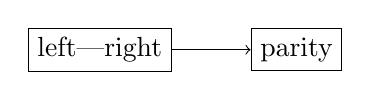
\begin{tikzpicture}
\node (a) [draw] {left|right};
\node (b) [draw, right=of a] {parity};
\draw[->] (a) -- (b);
\end{tikzpicture}
\end{document}
